\documentclass[12pt]{article}
\usepackage[parfill]{parskip}
\usepackage{amsmath}
\usepackage[nottoc,numbib]{tocbibind} % show bib in toc
\usepackage{graphicx}
\usepackage{hyperref}
\linespread{1.5}

\hypersetup{
    colorlinks,
    citecolor=black,
    filecolor=black,
    linkcolor=black,
    urlcolor=black
}

\bibliographystyle{plain}

\title{Perturbation theory and TQSSA}
\author{Oskar Thor\'{e}n}
\date{2015-04-18}

\begin{document}

\nocite{*} % include all references
\maketitle

\begin{abstract}
  Perturbation theory has a long history. In recent decades we have
  seen many applications in enzymatic kinetics. We start with some
  basic polynomial examples of regular perturbation theory, progress
  to singular perturbation and a boundary-value problem of
  differential equation, and then tackle a real application in the
  form of Total Quasi Steady State from enzyme kinetics.
\end{abstract}

\clearpage
\tableofcontents
\clearpage

\section{Introduction}

Perturbation theory has its roots in celestial mechanics and
aerodynamics. There are two particularly interesting victories that
perturbation theory has enabled. The first was the discovery of
Neptune, and the second was the theoretical foundation for
aerodynamics.

The promise of perturbation theory is that it allows us to find
approximate solutions to a larger class of problems, for example, in
differential equations, than we could otherwise with analytical
methods. It does this by giving us approximate but rigorous
solutions. In this article we will guide the reader from a very simple
and familiar example, a quadratic equation, all the way to a useful
research example in system biology: the total quasi steady state in
enzyme kinetics.

The article has been written with the goal that any student with a
basic understanding of calculus, differential equations and linear
algebra will be able to follow along. All the relevant biology and
perturbation theory will be explained as it becomes necessary.

\newpage
\section{A regular perturbation}

We are going to start with one of the simplest non-trivial examples
imaginable, a quadratic equation:
\begin{equation}
x^2 - 2x + \epsilon = 0.
\end{equation}
We know how to solve this analytically. The roots of the equation are\\
$x_1 = 1 + \sqrt{1 - \epsilon}$ and $x_2 = 1 - \sqrt{1 - \epsilon}$.

The case we are interested in is the one where $\epsilon$ is very
small. In this case, we can see that setting $\epsilon=0$ produces the
roots $x=0$ and $x=2$ respectively. In fact, for any given small
$\epsilon$ we notice that the solution changes very little. In that
sense it's a very "boring" and predictable problem.

Can we make more rigorous the observation that a small change in
$\epsilon$ only brings about a small change in the solution? One way
is to rewrite the part of the solution containing $\epsilon$ as a
\textit{Taylor series}. Recall the definition of a Taylor series for a
function $f(x)$ around a point a is
\begin{equation}
f(x) = \sum_{n=0}^{\infty} \frac{f^{n}(a)}{n!} (x-a)^n.
\end{equation}

The Taylor series for $f(\epsilon) = (1 - \epsilon)^{1/2}$ around 0
(since we assume that $\epsilon$ is very small) is thus
\begin{equation}
\sqrt{1 - \epsilon} = 1 - \frac{\epsilon}{2} - \frac{\epsilon^2}{8} + O(\epsilon^3),
\end{equation}
where $O(\epsilon^3)$ is some expression with a term $\epsilon^3$ in
it. This is called \textit{Big-Oh} notation and it is commonly used to
describe the limiting behaviour of a function. If we take the limit of
this expression as $\epsilon \to 0$, it's obvious that our intuition
is correct. That is, a small change in $\epsilon$ only brings about a
small change in the solution. We get
\begin{align}
x_1 &= 2 - \frac{\epsilon}{2} - \frac{\epsilon^2}{8} + O(\epsilon^3), \\
x_2 &= \frac{\epsilon}{2} + \frac{\epsilon^2}{8} + O(\epsilon^3).
\end{align}

What is the point of all this? We said in the beginning that
perturbation theory allows us to find approximate solutions to a
larger class of problems, but what we have done so far hasn't given
any indication of that being true. After all, we already have an
analytical formula for the quadratic equation.

Let's start over, but this time let's assume we don't have the
quadratic formula at our disposal. We will outline a method which
would allow us to get arbitrarly good approximations for polynomials
of any degree.

Let's assume the solutions of (1) in terms of x can be expressed in
the form of some power series of $\epsilon$, where $\epsilon$ is a
small number:
\begin{equation}
\sum_0^{\infty} a_k \epsilon^k = a_0 + a_1 \epsilon + a_2 \epsilon^2 + ...
\end{equation}
Another name for this type of series is \textit{perturbation series}.
We will now insert this perturbation series into (1), and then expand that
expression in terms of powers of $\epsilon$. We only have to do this
for the first few terms of the perturbation series to get a decent
approximation. If we want to we can always add more terms and get a
more accurate approximation. We have
\begin{equation}
(a_0 + a_1 \epsilon + a_2 \epsilon^2 + ...)^2 - 2(a_0 + a_1 \epsilon + a_2
\epsilon^2 + ...) + \epsilon = 0.
\end{equation}
We expand the expression using Big-Oh algebra. For example, for the
first term, we get: $(a_0 + a_1 \epsilon + a_2 \epsilon^2)^2 = a_0^2 +
2 a_0 a_1 \epsilon + (a_1^2 + 2 a_0 a_2) \epsilon^2 + O(\epsilon^3)$.
The whole expression becomes
\begin{equation}
a_0^2 - 2 a_0 + (2 a_0 a_1 - 2 a_1 + 1)\epsilon + (a_1^2 + 2 a_0 a_2 - 2 a_2)
\epsilon^2 = O(\epsilon^3), \epsilon \to 0.
\end{equation}

Now we turn to the problem of determining the coefficients $a_0$,
$a_1$ etc. Since $\epsilon$ is treated as a variable, as opposed to as
a parameter, we see that the coefficients before each power of
$\epsilon$ separately all have to be equal to zero. We thus get the
following system of equations for solving the coefficients:
\begin{align}
a_0^2 - 2 a_0 &=0, \\
2 a_0 a_1 - 2 a_1 + 1 &= 0, \\
a_1^2 + 2 a_0 a_2 - 2 a_2 &= 0.
\end{align}
Solving these equations in turn gives us, starting with the first
equation, $a_0 = 0$ or $a_0 = 2$. For $a_0 = 0$ we have $a_1 =
\frac{1}{2}$ and $a_2 = \frac{1}{8}$. For $a_0 = 2$ we have $a_1 = -
\frac{1}{2}$ and $a_2 = - \frac{1}{8}$.

We said at the beginning that we assume the solution is in the form of
a perturbation series. We have two options for the coefficients of
this perturbation series, and these corresponds to the two approximate
solutions of the original equation. From the above and (6) we get
\begin{align}
x_1 &= \frac{1}{2} \epsilon + \frac{1}{8} \epsilon^2 + O(\epsilon^3), \\
x_2 &= 2 - \frac{1}{2} \epsilon - \frac{1}{8} \epsilon^2 + O(\epsilon^3).
\end{align}
This is exactly the same as our previous solutions in (4) and (5),
without the use of the quadratic formula. There was nothing we did
that assumed a second degree polynomial. We have thus found a general
method for finding approximate solutions to polynomials of any degree
with a small parameter $\epsilon$.

\newpage
\section{A singular perturbation}

In the last section we dealt with a so called regular perturbation
problem. In this section we will deal with a singular perturbation
problem. What is the difference? In a singular perturbation problem,
the small $\epsilon$ \textit{matters} for the solution. In general,
singular problems are interesting precisely because their solutions
can change significantly with just a small change in
circumstances. More precisely, a singular perturbation problem is one
where setting $\epsilon$ to 0 doesn't give us a good approixmate
solution.

A way to get some intuition in the matter is to imagine balancing a
pen on a table. It's possible to get the pen to stay upright, but just
a slight perturbation of the pen results in it falling in one of many
directions.

As before, we will use a quadratic equation to illustrate how this
works,
\begin{equation}
\epsilon x^2 - 2 x + 1 = 0,
\end{equation}
where $\epsilon$ is a very small number. This equation has the
solutions
\begin{align}
x_1 &= \frac{1 + \sqrt{1 - \epsilon}}{\epsilon}, \\
x_2 &= \frac{1 - \sqrt{1 - \epsilon}}{\epsilon}.
\end{align}
The first thing we notice is that even though $\epsilon$ is very
small, we can't set it to zero. If we were to do it in (14), we would
only get a one degree polynomial. The fact that we are losing
solutions is a qualitative change and is indicative that we are
dealing with a singular perturbation problem.

Let's try using the same method as we did before. We assume x can be
expressed in the form of a perturbation series. Inserting this in our
equation gives us
\begin{equation}
\epsilon (a_0 + a_1 \epsilon + a_2 \epsilon^2)^2 - 2(a_0 + \epsilon a_1 +
a_2 \epsilon^2) + 1 = 0,
\end{equation}
which gets expanded into
\begin{equation}
(- 2 a_0 + 1) + (a_0^2 - 2 a_1) \epsilon + (2 a_0 a_1 -2 a_2) \epsilon^2 +
O(\epsilon^3),
\end{equation}
and leads to
\begin{align}
- 2 a_0 + 1 &= 0, \\
a_0^2 - 2 a_1 &= 0, \\
2 a_0 a_1 -2 a_2 &= 0.
\end{align}
The only solution to this system of equations is $a_0 = \frac{1}{2}$,
$a_1=\frac{1}{8}$, $a_2 = \frac{1}{16}$. This gives us only one of the
roots,
\begin{equation}
x_1 = \frac{1}{2} + \frac{1}{8} \epsilon + O(\epsilon^2).
\end{equation}
Note that the $a_2$ coefficient is included in the $O(\epsilon^2)$
expression. By the \textit{Fundamental Theorem of Algebra}, we would
expect to see two solutions. What happened to the other root? We
missed it because it's not on the form of a perturbation series. That
is, the other solution diverges as $\epsilon \to 0$. So what do we do?

The key here is that we can do a change in variable to turn the
problem into a regular perturbation problem:
\begin{equation}
x(\epsilon) = \frac{y(\epsilon)}{\delta(\epsilon)}.
\end{equation}
Here we are treating $x$ as a function, $y(\epsilon)$ is $O(1)$ and we want to
determine the re-scaling factor function $\delta(\epsilon)$. Our original
equation becomes
\begin{equation}
\frac{\epsilon}{\delta^2} y^2 - \frac{2}{\delta} y + 1 = 0.
\end{equation}
Our goal is to simplify this equation. We do this by dropping
insignificant terms. As we have seen, it turns out that the first term
in the equation is not insignificant, so we have to leave it in. Is
there some other term that we, to a first approximation, can drop?

All three terms in the above equation have some order of
magnitude. The method of dominant balance tells us to look for pairs
that balance ($\sim$), where balance means they are of the same order
of magnitude. We have already determined that the first term can't be
dropped, so we have two possibilities.

The first possibility is that $\frac{\epsilon}{\delta^2} y^2 \sim 1$,
with $\frac{2}{\delta}$ being insignificant.
$\frac{\epsilon}{\delta^2} = 1 \implies \delta =
\epsilon^{\frac{1}{2}}$.
But then $\frac{2}{\delta} = \frac{2}{\sqrt{\epsilon}}$ which isn't
small as $\epsilon \to 0$.

The second possibility is that
$\frac{\epsilon}{\delta^2} y^2 \sim \frac{2}{\delta} y$, with 1 being
insignificant. This means
$\frac{\epsilon}{\delta^2} = \frac{1}{\delta}$ which implies that
$\delta = \epsilon$. This seems correct as both expressions are
$O(\frac{1}{e})$, and 1 is small compared to this when
$\epsilon \to 0$. We get
\begin{align}
P(x) = \epsilon x^2 - 2x + 1, \\
\epsilon P\Big(\frac{y}{\epsilon}\Big) = y^2 - 2 y + \epsilon,
\end{align}
where the last part is exactly the same as our regular perturbation
problem in equation (1). As before, this gives us
\begin{align}
y_1 &= \frac{1}{2} \epsilon + \frac{1}{8} \epsilon^2 + O(\epsilon^3), \\
y_2 &= 2 - \frac{1}{2} \epsilon - \frac{1}{8} \epsilon^2 + O(\epsilon^3),
\end{align}
which means that
\begin{align}
x_1 &= \frac{1}{2} + \frac{1}{8} \epsilon + O(\epsilon^2), \\
x_2 &= \frac{2}{\epsilon} - \frac{1}{2} + \frac{1}{8} \epsilon + O(\epsilon^2).
\end{align}
The first root approaches $\frac{1}{2}$ as $\epsilon \to 0$, and the
second root is our missing solution that approaches $\infty$ as
$\epsilon \to 0$. This is the essence of singular perturbation theory
- to find the singular behavior and do a change of variable to turn it
into a regular perturbation problem.

\newpage
\section{ODE and boundary theory}

Boundary layer theory has its origins in aerodynamics and the work of
Prandtl. He discovered that fluids, like air around a plane and water
around some obstacle flow, are almost completely void of viscosity, or
stickiness, except for in a very thin region near the boundary of the
plane of the obstacle. This observation meant that one could treat
these two phenomena as separate problems - one where viscosity can be
discarded, and one where it matters a lot - as opposed to treating it
as one big complex problem. This simplified calculations greatly.

We will now give a basic example of this in the form of a
\textit{boundary value problem} with differential equations. Recall
that a boundary value problem is one where we have some set of
constraints that have to be fulfilled, called boundary conditions. We
will again look at a problem which we could solve explicitly, but
which we will instead use perturbation theory to analyze. In a
boundary value problem, we have two boundary value conditions and, in
a first approximation, they can't both be satisfied at the same
time. The strategy we use is to split the problem in two - one where
we are in a very thin region at $t=0$ (where we have a boundary
condition), the so called ``inner region'', and one where we are in an
``outer region'', which is everywhere else. This strategy is
generalizable to multiple layers.

We start by looking for the outer solution, then the inner solution,
then we match them together into one unified solution.

\subsection{Outer solution}

We are now going to look at a differential equation
\begin{equation}
\epsilon y'' + 2 y' + y, \enskip y(0)=0, \enskip y(1)=1, \enskip 0 < x < 1.
\end{equation}
If we naively set $\epsilon = 0$ we see that the resulting equation $2 y' + y$
has the general solution $C e^{- \frac{1}{2}x}$. This can't satisfy both
boundary conditions at once. If it satisfies $y(0)=0$ we have $y=0$ as the only
solution, and if it satisfies $y(1)=1$ we have
\begin{equation}
y_O=e^{\frac{1}{2} (1 - x)}.
\end{equation}
We are going to assume this is a good approximation somewhere. It is
valid for the $y(1)=1$ boundary condition, so we call this the
\textit{outer solution}.

Like the example in the last section, we missed something when we set $\epsilon
= 0$. We have found one of the two solutions and now we want to the find the
other one with the help of pairwise balancing.

\subsection{Inner solution}

We are assuming the boundary layer is near 0, and that it has a
thickness $\delta(\epsilon)$. By thickness we simply mean the order of
magnitude where the approximation is valid. For example, in Figure 2
(see section 4.4) we can see that at $x=\delta(\epsilon)=\epsilon$
(not derived until later in this section), the difference between the
approximation and the solution is negliable.

We introduce a re-scaling variable
\begin{equation}
\overline{x} = \frac{x}{\delta}.
\end{equation}
Having two scales like this is typical for singular perturbation problems. Our
original equation (31) becomes
\begin{equation}
\frac{\epsilon}{\delta^2} \frac{d^2y}{d\overline{x}^2} + \frac{2}{\delta}
\frac{dy}{d\overline{x}} + y = 0.
\end{equation}
We now do pairwise balancing, as before. Looking at the coefficients
of the above equation, we have the following orders of magnitude
\begin{equation}
O\Big(\frac{\epsilon}{\delta^2}\Big), O\Big(\frac{1}{\delta}\Big), O(1).
\end{equation}
We must have $\frac{\epsilon}{\delta^2}$ present, so the question is
if it balance one of the other terms with one being insignificant, and
if so, which one is insignificant. There are two possibilities. Either
we have
\begin{equation}
\frac{\epsilon}{\delta^2} \sim 1 \implies \delta = \epsilon^{\frac{1}{2}},
\end{equation}
but then $\frac{1}{\delta}$ is big compared to 1. Or we have
\begin{equation}
\frac{\epsilon}{\delta^2} \sim \frac{1}{\delta} \implies \delta = \epsilon,
\end{equation}
in which case 1 is indeed insignificant.

We have, multiplying by $\epsilon$, the inner equation
\begin{equation}
\frac{d^2 y}{d \overline{x}^2} + 2 \frac{dy}{d\overline{x}} + \epsilon
y = 0.
\end{equation}
To a first approximation we can neglect the last term, so we have
\begin{equation}
\frac{d^2 y}{d \overline{x}^2} + 2 \frac{dy}{d\overline{x}} = 0.
\end{equation}

Together with the other initial condition $y(0)=0$ we get the general inner
solution, valid in a region of thickness $\epsilon$ close to $x=0$,
\begin{equation}
y_I = C(1 - e^{-2\overline{x}}).
\end{equation}
We now have an outer and inner solution, and we turn to matching these
to determine the value of the constant $C$.

\newpage
\subsection{Matching and uniform approximation}
The idea behind \textit{matching} is that there is some edge or region
between the inner and outer solution, a region where both solutions
are valid approximations. We find a \textit{uniform approximation} by
piecing together our inner and outer solution, so that we have one
single expression of the solution that is valid everywhere in our
interval.

The procedure we will follow works in this case, but it's worth noting
that it's not always this straightforward. For more details, consult a
good textbook such as Bender and Orszag \cite{bender1999advanced}.

If we imagine a particle tracing the x-axis rightward, as we exit the boundary
layer, i.e. as $\overline{x} \to \infty$, the value of $y_I$ should be equal to
the value of $y_O$ as $x \to 0$, that is
\begin{equation}
\lim_{\overline{x} \to \infty} y_I = \lim_{x\to 0+} y_O \iff 
\lim_{\overline{x} \to \infty} C(1 - e^{-2\overline{x}}) = \lim_{x \to 0+} e^{\frac{1}{2}(1-x)}.
\end{equation}
This is called a \textit{matching condition}. The right-hand side equals
$e^{\frac{1}{2}}$, and thus the left-hand side gives us that $C =
e^{\frac{1}{2}}$.

We now have two separate approximations. We would like to have one
single approximation that is valid everywhere. We do this by adding
the two approximations together and removing their common part to
avoid double counting. Intuitively, one of the approximations is great
close to one of the boundary conditions, ok in the middle, and
terrible close to the other boundary conditions. The other
approximation is exactly the opposite. By combining them, we get a
smooth approximation of the whole solution:
\begin{equation}
y_U = y_o(x) + y_I\Big(\frac{x}{\delta}\Big) - e^{\frac{1}{2}}.
\end{equation}
The common part comes from the matching condition earlier in this
section. In the inner region the other terms are negliable, and vice
versa in the outer region,
\begin{align}
  y_U &= e^{\frac{1}{2}(1-x)} + e^{\frac{1}{2}}(1 - e^{\frac{-2x}{\epsilon}}) -
        e^{\frac{1}{2}} \\
      &=  e^{\frac{1}{2}}(e^{\frac{-x}{2}} - e^{\frac{-2x}{\epsilon}}).
\end{align}
This is our uniform approximation for the whole solution. We can
compare this to the exact solution and see that it is indeed a good
approximation.

\subsection{Comparison with exact solution}

We saw in the previous section what a good approximation to the
solution is. Our original equation (31) can however be solved exactly,
so let's do that.

The \textit{characteristic polynomial} $\epsilon r^2 +2r + 1 = 0$ has
the solutions $\frac{-1 \pm \sqrt{1-\epsilon}}{\epsilon}$. We have
that
\begin{equation}
y_{\epsilon}(x)=c_1 e^{\frac{-1 + \sqrt{1-\epsilon}}{\epsilon} x} + c_2
e^{\frac{-1 - \sqrt{1-\epsilon}}{\epsilon} x}.
\end{equation}
With the help of the boundary conditions $y(0)=0, y(1)=1$ we see that
\begin{equation}
  c_2 = - c_1 = - \frac{1}{e^{\frac{-1 + \sqrt{1-\epsilon}}{\epsilon}}
    - e^{\frac{-1 - \sqrt{1-\epsilon}}{\epsilon}}}.
\end{equation}
We use a Taylor expansion as before and define
\begin{align}
  \alpha_1 &= \frac{1 - \sqrt{1-\epsilon}}{\epsilon} = \frac{1}{2} + O(\epsilon), \\
  \alpha_2 &= 1+ \sqrt{1-\epsilon} = 2 + O(\epsilon).
\end{align}
We can then express the solution as
\begin{equation}
  y_{\epsilon}(x) = \frac{1}{e^{-\alpha_1(\epsilon)} - e^{\frac{-\alpha_2(\epsilon)}{\epsilon}}} \Big(e^{-\alpha_1(\epsilon)x} - e^{\frac{-\alpha_2(\epsilon)x}{\epsilon}}\Big).
\end{equation}
There are two terms in this solution. As $\epsilon \to 0+$, for fixed
$x \in (0,1)$, all the expressions involving division by $\epsilon$
disappear, i.e. all the $a_2$ terms. The solution becomes
\begin{equation}
  y_{\epsilon}(x) \to \frac{e^{\frac{-x}{2}}}{e^{\frac{-1}{2}}} = e^{\frac{1}{2}(1-x)}.
\end{equation}
This is exactly the outer solution we got before in (32), satisfying
$y(1)=1$ but not $y(0)=0$.

Notice that the above is just valid for a fixed x, as we will see
below. If we instead take (49) and notice that, for arbitrarily small
$\epsilon$, $e^{-\frac{\alpha_2(\epsilon)}{\epsilon}}$ is 0. The exact
solution is thus (we distinguish between an approximation of the exact
solution, and the outer approximation):
\begin{equation}
  y_{\epsilon}(x) \approx e^{\frac{1}{2}}(e^{-\frac{x}{2}} -
  e^{-\frac{2x}{\epsilon}}), \quad 0 < \epsilon \ll 1.
\end{equation}

When we graph (50) and (51) for any given $\epsilon$ we see that,
outside of a small region near 0, the outer approximation is indeed a
good approximation. We get the second graph by doing the same thing
for the inner solution.

For the first graph, note that the outer approximation starts at
$y(0)=e^{\frac{1}{2}}$, and thus misses the contribution $\epsilon$
has on the solution for very small x values.

For the second graph, notice the agreement between the exact and inner
approximation in a region close to $x=0$ (which we can move
arbitrarily closer by using a smaller $\epsilon$).

\newpage
\begin{figure}[ht!]
\centering
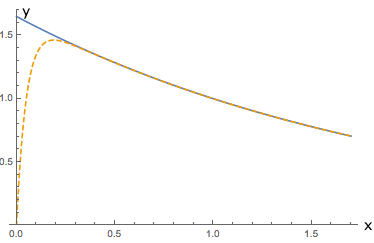
\includegraphics[width=120mm]
{tmp_ode-outer_axis.png}
\caption{The full line is the outer approximation, $\epsilon=0.1$.}
\label{overflow}
\end{figure}

\begin{figure}[ht!]
\centering
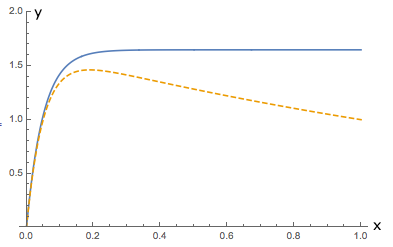
\includegraphics[width=120mm]
{tmp_ode-inner_axis.png}
\caption{The full line is the inner approximation, $\epsilon=0.1$.}
\label{overflow}
\end{figure}

\section{Total Quasi Steady State}
\subsection{A biological problem}

In enzyme kinetics we often come across chemical reactions like
\begin{equation}
E + S \underset{k_{-1}}{\overset{k_{1}}\rightleftharpoons} C
 \overset{k_2}\longrightarrow E + P
\end{equation}
This is an enzyme E and substrate S that combine, reversibly, to form
a complex C, which in turn gives us a product P and enzyme E back.
$k_1, k_{-1}, k_2$ are rate constants. We won't bother with the
biological details too much, but will instead look at how we can
analyze the above as a dynamical system.

The \textit{law of mass action} tells us that two molecules A and B
forming complex C, $A+B \overset{k}\longrightarrow C$ are governed by
$\frac{dC}{dt} = kAB$. That is, the greater concentration of A or B we
have, the faster the complex C is formed. This has been
experimentally verified by Guldberg and Waage in 1867, and many times
since.

With this law, we can translate our chemical reaction into a system of
differential equations:
\begin{align}
\frac{dE}{dt} &= -k_1ES + k_{-1}C + k_2C, \\
\frac{dS}{dt} &= -k_1ES + k_{-1}C, \\
\frac{dC}{dt} &= k_1ES - k_{-1}C - k_2C, \\
\frac{dP}{dt} &= k_2C.
\end{align}
In the study of enzyme kinetics, we normally have some initial conditions to help
us out: $S(0) = S_0, E(0) = E_0, C(0)=0, P(0)=0$.

We see immediately that
\begin{equation}
\frac{dE}{dt} + \frac{dC}{dt} = 0.
\end{equation}
Together with the initial conditions we get that
\begin{equation}
E + C = E_0,
\end{equation}
which we can use to eliminate E from the equation. This is called a conservation
law.  We also don't care about P, as it doesn't feed back into the other
equations. We are left with
\begin{align}
\frac{dS}{dt} &= -k_1(E_0 - C)S + k_{-1}C, \\
\frac{dC}{dt} &= k_1(E_0 - C)S - k_{-1}C - k_2 C.
\end{align}
This is a two-dimensional system, which is much easier to deal with. Can we do
better? It turns out we can.

Very often, in practice, the substrate has a much higher concentration
than the enzyme. This means that C can be treated as constant after a
short initial period. By exploiting this fact, we can reduce the
system to one equation. This is called the \textit{Quasi-Steady State
  approximation}.

Assume that C is constant $\iff \frac{dC}{dt} = 0$ after a short
period of time. Then we write
\begin{equation}
\frac{dS}{dt} = -k_2 C
\end{equation}
with
\begin{equation}
C = \frac{E_0 S}{K_m +S},
\end{equation}
where $K_m = \frac{k_{-1} + k_2}{k_1}$ is the so called {Michaelis-Menten
constant}. We have
\begin{equation}
\frac{dS}{dt} = - \frac{k_2 E_0 S}{K_m + S}
\end{equation}
together with $S(0) = S_0$ as initial condition. This is what is
normally considered the QSSA, valid after some short amount of time
has passed.

We can justify this with a procedure similar to one in the previous
section, as done by for example Lin and Segel
\cite{lin1974mathematics}. Instead we are going to look at a slight
variation of this, namely what happens when the amount of substrate
isn't much bigger than the amount of enzyme. This is the
\textit{Total Quasi Steady State assumption}, discovered by Borghans
and Segel 1996 \cite{borghans1996extending}.

\subsection{TQSSA}

The basic idea behind TQSSA is to perform a change of variable
\begin{equation}
\overline{S} = S + C.
\end{equation}
This change of variable makes the approximation valid not just when
the substrate has a much higher concentration than the enzyme, but
also, under certain conditions, when they are roughly equal. This
makes the TQSSA valid for a wider range of parameters. We will see in
the next few sections what those conditions are.

We get the following system of equations from (59), (60) and (64)
\begin{align}
\frac{d\overline{S}}{dt} &= - k_2 C, \\
\frac{dC}{dt} &= k_1(E_0-C)(\overline{S}-C)-(k_{-1}+ k_2) C.
\end{align}
Together with initial conditions $\overline{S}(0)=S_0, C(0)=0$, these
are the rate equations for the TQSSA.
\begin{figure}[ht!]
\centering
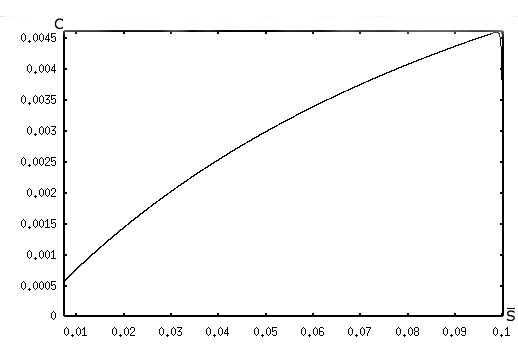
\includegraphics[width=120mm]
{tqssa-phase-plane-b_axis.png}
\caption{TQSSA phase plane. Initial state is $\overline{S}(0)=0.1,
  C(0)=0$. $E=0.01, k_1=10, k_{-1}=1, k_2=0.1$.}
\label{overflow}
\end{figure}

We get some intuition of the behavior by inspecting the phase plane of
the above equations. With the help of XPP (see appendix for the source
code used), we can numerically simulate the system, as seen in Figure
3. There are two things to note: (1) the steady state is at (0,0) (not
shown in graph due to numerical rounding error, but this can easily be
seen looking at the equations above) and (2) from the initial state
there's a rapid increase of concentration in the complex C, after
which it slowly decreases (quasi-steady state) until it reaches steady
state

The rapid increase of concentration in the complex C is just barely
visible in the top right corner. It can also be seen by looking at the
initial conditions, and then noticing that right after that the line
is in the top right corner.

\subsection{Timescales}

To analyze the problem rigorously using perturbation theory, we need
to find an expression that estimates these two time scales that the
system is operating with, $t_C$ for the fast initial period and
$t_{\overline{S}}$ for the slow quasi-steady state period.

One way to get some intuition behind the use of different time scales
is to think about the difference between seconds and years. Some
phenomena happens on the scale of seconds or less, like many chemical
reaction, whereas the development of cities happens on a scale of
years. If you blink, the city landscape isn't going to change before
your eyes. Using different time scales is a way to capture that
observation in a rigorous fashion.

We are first going to calculate the timescales for the normal QSSA, to
get some intuition for the concept. We will then extend this to the
TQSSA. Exactly why these timescales are good is not obviously, but as
we move into the next section on Scaling the reasons will hopefully
become more clear. Essentially it's about finding good approximations
for when the (T)QSSA is valid.

To get the fast time scale, we can estimate S as $S_0$ since in that
time period the substrate concentration won't change much and we just
care about rough orders of magnitudes for the timescales. From (60) we
get
\begin{equation}
  \frac{dC}{dt} = k_1E_0 S_0 - (k_1 S_0 + k_{-1} + k_2)C.
\end{equation}
With the help of the initial condition $C(0)=0$, we get the solution
\begin{equation}
  C(t) = A(1 -  e^{\lambda x}), \quad
  \lambda = (-S_0 k_1 + k_{-1} + k_2), \quad
  A =\frac{k_1 E_0 S_0}{S_0 k_1 + k_{-1} + k_2}.
\end{equation}
The timescale here is $t_C = |\lambda^{-1}|$, which we can rewrite as
\begin{equation}
  t_C = \frac{1}{k_1(S_0+K_m)}.
\end{equation}

To get the other time scale we first use that $dC/dt = 0$ after some
period of time, which is the time period we care about. We get $t_s$
with the help of an estimation technique by Segel
\cite{segel1984modeling}. This technique tells us to take
$S_{\max} - S_{\min} = S_0$ divided by the maximum of $|dS/dt|$ using
$S=S_0$ in (63). This gives us
\begin{align}
  t_s &= \frac{S_{\max} - S_{\min}}{|dS/dt|_{\max}} \\
      &= \frac{K_m + S_0}{k_2 E_0}.
\end{align}

So far we have only derived timescales for the normal QSSA. To get the
timescales for TQSSA, we use the substitution from (64). By doing so,
and assuming $\frac{dC}{dt}=0$ as before, (66) becomes
\begin{equation}
  C^2 - (E_0 + K_m + \overline{S})C + E_0 \overline{S} = 0.
\end{equation}
We define a function f with the goal of solving for C as
\begin{align}
  f(C) &= C^2 - (E_0 + K_m + \overline{S})C + E_0 \overline{S}.
\end{align}

If we have a quadratic equation $x^2+bx+c$, assuming there are two
roots $x_1$ and $x_2$, then the quadratic equation can be factored
into $(x - x_1)(x - x_2)$, where
\begin{equation}
  x_1 x_2 = c.
\end{equation}

Is there a unique positive solution to (74)? No. We know
$f(0) = E_0 \overline{S} > 0$, since a concentration can never be less
than 0, and we know from the above identity that
$c_1 c_2 = E_0 \overline{S}$. Thus, assuming $c_1$, $c_2$ are
solutions, $c_1 c_2 > 0$, which in turn implies that both roots are
positive or both roots are negative.

Are there positive solutions? Yes. We have:
\begin{align}
  f(0) &= E_0 \overline{S} > 0, \\
  f(E_0) &= E_0^2 - (E_0 + K_m + \overline{S})E_0 + E_0 \overline{S} \\
         &= - K_m E_0 < 0.
\end{align}

Using the Intermediate Value Theorem for continuous functions, there
must be a number $c_1 \in (0,E_0)$, such that $f(c_1) = 0$ is a
solution. Moreover, since we are dealing with a real polynomial, the
Complex Conjugate Root Theorem says that the complex roots appear in
pair. Together with what we saw above, this implies that both $c_1$
and $c_2$ are positive.

With this we get the following inequalities. First, the discriminant
of f(c) is positive:
\begin{equation}
  (E_0 + K_m + \overline{S})^2 - 4 E_0 \overline{S} > 0.
\end{equation}

For a quadratic equation $x^2 + bx + c$, we have another identity for
its roots:
\begin{align}
  x_1 + x_2 &= \frac{-b + \sqrt{b^2-4c}}{2} + \frac{-b - \sqrt{b^2-4c}}{2} = -b.
\end{align}

Hence
\begin{align}
  c_1 + c_2 = E_0 + K_m + \overline{S} \iff c_2 = E_0 + K_m + \overline{S} - c_1.
\end{align}

And we have our second set of inequalities:
\begin{align}
  c_1 &< E_0 &\implies c_2 &> K_m + \overline{S}, \\
  c_1 &> 0 &\implies c_2 &< E_0 + K_m + \overline{S}.
\end{align}

With these inequalities, we can position the roots as follows:
\begin{align}
  0 &< c_1 < E_0, \\
  0 < K_m + \overline{S} &< c_2 < E_0 + K_m + \overline{S}.
\end{align}

If $E_0 < K_m + \overline{S}$ there is only one solution that
satisfies the conservation law (58), since for $c_2$ we would have a
contradiction (since E can't be negative):
\begin{align}
  0 < E_0, \enskip E_0 &= E + c_2, \\
  E_0 < K_m + \overline{S} < c_2 &\implies E < 0.
\end{align}

Assuming that the condition above holds, we thus have as our only solution
\begin{equation}
  c_1(\overline{S}) = \frac{E_0 + K_m + \overline{S} - \sqrt{(E_0 +
      K_m + \overline{S})^2 - 4 E_0 \overline{S}}}{2}.
\end{equation}

We want to investigate what happens when $\overline{S}$ is very
large. Multiplying both sides with the conjugate we get
\begin{align}
  c_1(\overline{S}) &= \frac{E_0 \overline{S}}{E_0 + K_m + \overline{S} +
    \sqrt{(E_0 +K_m + \overline{S})^2 - 4 E_0 \overline{S}}}, \\
                    &= \frac{2 E_0}{\frac{E_0 + K_m}{\overline{S}} + 1 +
    \sqrt{(\frac{E_0 + K_m}{\overline{S}} + 1)^2 - \frac{4 E_0}{\overline{S}}}}
  \to  E_0 \enskip \text{as} \enskip \overline{S} \to \infty.
\end{align}
% Our approximation must have the property that c_1(barS) -> E_0

Since we always have that
$(E_0 + K_m + \overline{S})^2 \geq E_0 \overline{S}$ we can rewrite (89),
\begin{align}
  c_1 &= \frac{2 E_0 \overline{S}}
              {(E_0 + K_m + \overline{S}) + (E_0 + K_m + \overline{S})
              \sqrt{1- \frac{4 E_0 \overline{S}}
                            {(E_0 + K_m + \overline{S})^2}}} \\
      &= \frac{2 E_0 \overline{S}}
              {\Big(E_0 + K_m + \overline{S}\Big)
              \Big(1 + \sqrt{1- \frac{4 E_0 \overline{S}}
                  {(E_0 + K_m + \overline{S})^2}}\Big)}.
\end{align}

Recall that for an expression like $\sqrt{1-x}$ the Taylor expansion
around $x=0$ is $1 - O(x)$. This converges for $|x| < 1$. In our case
that means we can simplify the above as
\begin{align}
   c_1 &= \frac{2 E_0 \overline{S}}
              {\Big(E_0 + K_m + \overline{S}\Big)
               \Big(1 + \Big(1 -
                O\Big(\frac{4 E_0 \overline{S}}
                           {(E_0 + K_m + \overline{S})^2}\Big)\Big)\Big)} \\
      &\approx \frac{E_0 \overline{S}}
                    {E_0 + K_m + \overline{S}}.
\end{align}

Let's now look at when the following inequality holds
\begin{equation}
(E_0 + K_m + \overline{S})^2 \gg E_0 \overline{S}.
\end{equation}
This is equivalent to
\begin{align}
1 \ll
  \frac{(E_0 + K_m + \overline{S})^2}
           {E_0 \overline{S}} &= 
\frac{(E_0 + K_m + \overline{S})}
      {E_0} \frac{(E_0 + K_m + \overline{S})}{\overline{S}} \\
&= \Big(1 + \frac{K_m}{E_0} + \frac{\overline{S}}{E_0}\Big)
   \Big(1 + \frac{E_0}{\overline{S}} + \frac{K_m}{\overline{S}}\Big).
\end{align}
This is true both when $\overline{S}$ is sufficiently large and when
it is sufficiently small compared to $E_0$.

If $\overline{S} = E_0$ then
\begin{equation}
\Big(1 + \frac{K_m}{E_0} + \frac{\overline{S}}{E_0}\Big)\Big(1 + \frac{E_0}{\overline{S}} + \frac{K_m}{\overline{S}}\Big) = \Big(2 + \frac{K_m}{E_0}\Big) \Big(2 + \frac{K_m}{E_0}\Big) \gg 1.
\end{equation}

So if $E_0 < K_m + \overline{S}$ our approximation (94) is possible.

Doing calucations similar to what we did in beginning of this section,
using equation (94), we eventually end up with these two slightly
modified time-scales:
\begin{align}
t_C &= \frac{1}{k_1(E_0+S_0+K_m)}, \\
t_{\overline{S}} &= \frac{E_0+S_0+K_m}{k_2+E_0},
\end{align}
with $K_m = \frac{k_{-1}+k_2}{k_1}$ as before. We will now analyze
this problem like we did in section 4. But first, we have to
scale the system using our newly discovered timescales.

\subsection{Scaling}

Lin and Segel defines \textit{scaling} as follows:

\textit{Scaling amounts to nondimensionalizing so that relative magnitude of
each term is indicated by a dimensionless factor preceding that term}
\cite{lin1974mathematics}.

We will now introduce scaled, dimensionless variables. We get these
variables by dividing by their respective scales. We have the two time
variables
\begin{align}
\tau &= \frac{t}{t_C}, \\
T &= \frac{t}{t_{\overline{S}}},
\end{align}
where $\tau$ is the fast time scale, and $T$ the slow one. We also
scale C and $\overline{S}$ by their maximum:
\begin{align}
c &= \frac{C}{C_0}, \\
s &= \frac{\overline{S}}{S_0}.
\end{align}
$S_0$ is max since S starts from some constant value $S_0$ and then
turns into the complex C, as we saw before. We derive C's max, $C_0$,
by using the approximation we got for C in (94) and $S=S_0$:
\begin{equation}
C_0 = \frac{E_0 S_0}{E_0 + S_0 + K_m}.
\end{equation}

\subsection{Outer solution}

Now we need a small parameter $\epsilon$ to begin looking for the
outer solution, when the complex changes slowly. A necessary condition
for the TQSSA to hold is $0 < \epsilon \ll 1$ where
\begin{equation}
\epsilon = \frac{t_C}{t_{\overline{S}}} = \frac{k_2 E_0}{k_1(E_0+S_0+K_m)^2}.
\end{equation}

This comes from Borghans, and it makes sense given what we have
learned about timescales - you can only treat a city landscape as
static if you are looking at it on a short timescale. Assuming
$t_C \ll t_{\overline{S}}$ we will calculate for the outer region,
using the procedure by Khoo and Heglund
\cite{khoo2008total}. Translating equation (65) and (66) with the help
of the above equations and the chain rule,
\begin{equation}
\frac{dc}{dT} = \frac{dC}{dt} \enskip \frac{dt}{dT} \enskip \frac{dc}{dC},
\end{equation}
we get
\begin{align}
\frac{dc}{dT} &= \frac{t_{\overline{S}}}{C_0}
       \Big[k_1 \Big(E_0 S_0 s - (E_0 + S_0 s + K_m) C_0 c + (C_0 c)^2
                   \Big)\Big] \\
              &= \frac{(E_0+S_0+K_m)^2 k_1}{(k_2 + E_0)}
                 \Big(s - \frac{E_0+S_0 s+K_m}{E_0 + S_0 + K_m} c
                        + \frac{(C_0)^2}{E_0 S_0} c^2 \Big) \\
              &= \frac{1}{\epsilon}
                 \Big(s - \frac{E_0+S_0 s+K_m}{E_0 + S_0 + K_m} c
                        +  \gamma c^2 \Big)
\end{align}
with
\begin{equation}
\gamma = \frac{(C_0)^2}{E_0 S_0} = \frac{E_0 S_0}{(E_0 + S_0 + K_m)^2}.
\end{equation}

We now have an equation of the form
\begin{equation}
  \epsilon \frac{dc}{dT} = \gamma c^2 - \frac{E_0+S_0 s+K_m}{E_0 + S_0 + K_m} c+ s.
\end{equation}
We also note that as $\gamma \to 0$, $\epsilon \to 0$.

Similarly to what we saw in Section 3, as $\epsilon \to 0$, we have that
\begin{equation}
   \gamma c^2  - \frac{E_0+S_0 s+K_m}{E_0 + S_0 + K_m} c + s = 0.
\end{equation}

As justified in (95) to (98), $\gamma \ll 1$ when $\overline{S}$ is
sufficiently large or small compared to $E_0$. Recall what we learned
in Section 3. We have established that, under certain conditions, the
quadratic equation has only one solution. Our above quadratic is, to a
first approximation, thus
\begin{equation}
  s - \frac{E_0+S_0 s+K_m}{E_0 + S_0 + K_m} c = 0.
\end{equation}

Thus we obtain our outer solution (note the subscript 'O' as in the
author's first name):
\begin{equation}
  c_O = \frac{E_0 + S_0 + K_m}{E_0+S_0 s+K_m} s.
\end{equation}

If we substitute this into equation (65), after scaling for the slow
timescale, we get an expression for the outer solution of s:
\begin{equation}
\frac{ds}{dT} = - \frac{E_0 + S_0 + K_m}{E_0 + S_0s + K_m}s, \enskip s(0) = 1.
\end{equation}

We can solve this by separation of variables:
\begin{equation}
\int \frac{E_0 + S_0 s + K_m}{(E_0 + S_0 + K_m) s} ds = \int - dT.
\end{equation}
The left hand side is an equation of the form:
\begin{align}
&\int \frac{a + b x + c}{(a + b + c) x} dx
        \quad \text{[u = a + bx + c]} \\
&\iff \frac{1}{a+b+c} \int \frac{u}{u - a -c} du \\
&\iff \frac{1}{a+b+c} \int \Big(\frac{a+c}{u - a -c} + 1\Big)
                          du \\
&\iff \frac{a+c}{a+b+c} \int \frac{1}{u - a - c} du
                    + \frac{1}{a+b+c} \int 1 du \\
&\iff \frac{(a+c) \ln{x}}{a+b+c} + \frac{bx}{a+b+c} + \text{constant}.
\end{align}

This makes the solution to (117)
\begin{equation}
\frac{E_0+K_m}{E_0 + S_0 + K_m} \ln{s} + \frac{S_0}{E_0 + S_0 + K_m} s = - T + \text{constant}.
\end{equation}

Using the initial condition $s(0)=1$, and the fact that $t=0$, we get
the constant
\begin{equation}
  \frac{S_0}{E_0 + S_0 + K_m}.
\end{equation}

This gives us the outer solution for s, $s_O$:
\begin{equation}
  (E_0+K_m) \ln{s_O(T)} + S_0 (s_O(T) - 1) + (E_0 + S_0 + K_m) T = 0.
\end{equation}

\subsection{Inner solution}

The outer solution can't satisfy the initial conditions for our
problem, which is why we have an inner solution where the complex
changes quickly. Proceeding as with the outer solution, we scale (65):
\begin{align}
\frac{ds}{d\tau} &= \frac{t_C}{S_0} \Big( - k_2 C_0 c \Big) \\
                 &= \frac{-k_2 E_0}{k_1(E_0 + S_0 + K_m)^2} c \\
                 &= \epsilon c.
\end{align}

As $\epsilon \to 0$, the above becomes $\frac{ds}{d\tau} = 0$. That
is, s is approximately constant at this fast time scale. Together with
the initial condition $s(0)=1$, we have the inner solution for s
\begin{equation}
s_I(\tau) = s(0) = 1.
\end{equation}

For c we get, using $s= s_I = 1$,
\begin{align}
\frac{dc}{d\tau} &= \frac{t_C}{C_0} \Big(
                     k_1 E_0 S_0 s - k_1 C_0 (E_0 + S_0 s + K_m) c + k_1 C_0^2 c^2
                     \Big) \\
                 & = - \gamma c^2 - c + 1.
\end{align}
We solve this by separation of variables, like before:
\begin{equation}
\frac{dc}{- \gamma c^2 - c + 1} = d\tau.
\end{equation}

By B\'{e}zout's identity for polynomials, there exists polynomials $C$
and $D$ such that
\begin{equation}
\frac{1}{P(x) Q(x)} = \frac{C}{Q(x)} + \frac{D}{P(x)},
\end{equation}
where $CP+DQ = 1$. We will use this in the partial fraction step below.

Let $\Delta=1 + 4\gamma$. We investigate the denominator in (132):
\begin{align}
&-\gamma c^2 - c + 1 = - \gamma
                        \Big(c - \frac{-1 + \sqrt{\Delta}}{2 \gamma}\Big)
                        \Big(c + \frac{ 1 + \sqrt{\Delta}}{2 \gamma}\Big) \\
&\implies \frac{1}{- \gamma c^2 - c + 1} = \frac{1}
                        {- \gamma
                        \Big(c - \frac{-1 + \sqrt{\Delta}}{2 \gamma}\Big)
                        \Big(c + \frac{ 1 + \sqrt{\Delta}}{2 \gamma}\Big)} \\
&= - \frac{1}{\sqrt{\Delta}}
   \Bigg(\frac{1}{c - \frac{-1 + \sqrt{\Delta}}{2 \gamma}} -
        \frac{1}{c + \frac{1 + \sqrt{\Delta}}{2 \gamma}} \Bigg)
   \quad \text{(see above identity)}.
\end{align}

Integrating (132) we get
\begin{align}
&\frac{-1}{\sqrt{\Delta}}
\Big( \int \frac{dc}{c - \frac{\sqrt{\Delta} - 1}{2 \gamma}} -
      \int \frac{dc}{c + \frac{\sqrt{\Delta} + 1}{2 \gamma}}
\Big) = \tau + \text{constant} \\
&\iff \frac{-1}{\sqrt{\Delta}}
      \ln \bigg|\frac{c - \frac{\sqrt{\Delta}-1}{2\gamma}}
                     {c + \frac{\sqrt{\Delta}+1}{2\gamma}} \bigg|
 = \tau + \text{constant} \\
&\iff \frac{1}{\sqrt{\Delta}}
      \ln \bigg|\frac{c + \frac{\sqrt{\Delta}+1}{2\gamma}}
                     {c - \frac{\sqrt{\Delta}-1}{2\gamma}} \bigg|
 = \tau + \text{constant} \\
&\iff  \ln \bigg|\frac{2\gamma c + \sqrt{\Delta}+1}
                      {2\gamma c - \sqrt{\Delta}+1} \bigg|
 = (\tau + \text{constant}) \sqrt{\Delta}.
\end{align}

Note that $|-\sqrt{\Delta}+1| = \sqrt{\Delta} - 1$. $c(0)=0$ makes the constant
\begin{equation}
\frac{1}{\sqrt{\Delta}} \ln \frac{\sqrt{\Delta}+1}{{\sqrt{\Delta}-1}},
\end{equation}
which gives us
\begin{align}
&\ln \bigg|\frac{2\gamma c + \sqrt{\Delta}+1}
                {2\gamma c - \sqrt{\Delta}+1} \bigg|
 = \tau \sqrt{\Delta} + \ln \frac{\sqrt{\Delta}+1}{{\sqrt{\Delta}-1}}\\
&\implies \bigg|\frac{2\gamma c + \sqrt{\Delta}+1}
                     {2\gamma c - \sqrt{\Delta}+1} \bigg|
 = \frac{\sqrt{\Delta}+1}{{\sqrt{\Delta}-1}} \mathrm{e}^{\sqrt{\Delta} \tau}.
\end{align}

Note that $2 \gamma c + \sqrt{\Delta} + 1 > 1 > 0$ and
$2 \gamma c - \sqrt{\Delta} + 1 < 0$. That the second inequality is
true is not obvious, but we will see that this is indeed the case in
the next section.

We then have:
\begin{align}
&(2\gamma c + \sqrt{\Delta} + 1)(\sqrt{\Delta} - 1) =
   (\sqrt{\Delta} - 2\gamma c - 1)(\sqrt{\Delta} + 1) e^{\sqrt{\Delta} \tau} \\
&\iff 2\gamma c (\sqrt{\Delta} - 1) + 4 \gamma =
  \Big( -2\gamma c(\sqrt{\Delta} + 1) + 4\gamma \Big) e^{\sqrt{\Delta} \tau} \\
&\iff c (\sqrt{\Delta} - 1) + c (\sqrt{\Delta} + 1) e^{\sqrt{\Delta} \tau} =
   2(e^{\sqrt{\Delta} \tau} - 1) \\
&\implies c_I(\tau) =
  \frac{2(e^{\sqrt{\Delta} \tau} - 1)}
       {  (\sqrt{\Delta} + 1) e^{\sqrt{\Delta} \tau} + (\sqrt{\Delta} - 1)} \\
&\iff c_I(\tau) =
  \frac{2(e^{\sqrt{1+4\gamma} \tau} - 1)}
       {(\sqrt{1+4\gamma} + 1) e^{\sqrt{1+4\gamma} \tau} + \sqrt{1+4\gamma} - 1},
\end{align}
which is our inner solution for c. Note that this is a different
result from what Khoo and Heglund got. It seems as if their result is
incorrect.

\subsection{Matching and uniform approximation}

As before in section 4.3, we are looking for a common limit, and our
matching condition as
$\epsilon \to 0 \text{, } \tau \to \infty \text{, and } T \to 0$ is
\begin{equation}
\lim_{\epsilon \to 0} [y_O(T) |_{T=0}] =
\lim_{\epsilon \to 0} [y_I(\tau) |_{\tau=\infty}].
\end{equation}

For the substrate s this is
\begin{align}
&\lim_{\epsilon \to 0} [s_O(T) |_{T=0}] =
  \lim_{\epsilon \to 0} [s_I(\tau) |_{\tau=\infty}] \\
&\iff \lim_{\epsilon \to 0} [s_O(T) |_{T=0}] =
  \lim_{\epsilon \to 0} 1.
\end{align}

We don't have an explicit expression for $s_O$, but the right hand
side above is obviously 1, and evaluating the implicit expression for
$s_O(0)$ from (125) we see that $s_O(0)=1$ is indeed a solution:
\begin{equation}
(E_0+K_m) \ln{s_O(0)} + S_0 (s_O(0) - 1) = 0.
\end{equation}

The matching condition in (149) is thus simply equal to 1.

For the complex c we have
\begin{equation}
\lim_{\epsilon \to 0} [c_O(T) |_{T=0}] =
  \lim_{\epsilon \to 0} [c_I(\tau) |_{\tau=\infty}].
\end{equation}

For $c_O(T)$ at $T=0$ we have
\begin{align}
c_O(0) &= \frac{E_0 + S_0 + K_m}{E_0+S_0 s(0) +K_m} s(0) \\
       &= \frac{E_0 + S_0 + K_m}{E_0+S_0  +K_m} \\
       &= 1 \text { as } \epsilon \to 0.
\end{align}

As we established earlier, $\gamma \ll 1$.We use this to proceed
similarly to how we did in (92) to (94), and approximate the
expression $\sqrt{1+4\gamma}$ as $1+O(1+4\gamma) \approx 1$ as
$\gamma \to 0$. We then have for $c_I(\tau)$:
\begin{align}
c_I(\tau) &=
     \frac{2(e^{\sqrt{1+4\gamma} \tau} - 1)}
   {(\sqrt{1+4\gamma} + 1) e^{\sqrt{1+4\gamma} \tau} + \sqrt{1+4\gamma} - 1} \\
&= \frac{2(e^{(1+O(1+4\gamma)) \tau} - 1)}
        {(2 + O(1+4\gamma)) e^{(1+O(1+4\gamma)) \tau} + O(1+4\gamma)} \\
&\approx \frac{2(e^{\tau} - 1)}
              {(2 + O(1+4\gamma)) e^{\tau}} \\
&= \frac{2(1 - \frac{1}{e^{\tau}})}
        {2 + O(1+4\gamma)} \\
&= \frac{2(1 - \frac{1}{e^{\tau}})}
        {1 + \sqrt{1+4\gamma}}
   \to \frac{2} {1 + \sqrt{1+4\gamma}} \quad \text{as } \tau \to \infty.
\end{align}

Even though the expressions for $c_O$ and $c_I$ look different, they
are both equal to 1 in the limiting case as (161) $\to 1$ as
$\tau \to 0$ and $\gamma \to 0$. This corresponds to how well the
TQSSA approximation works. Note that this would not be the case if we
chose differently in the inequality after equation (142). Equation
(153) is thus
\begin{equation}
\approx \frac{2} {1 + \sqrt{1+4\gamma}}.
\end{equation}

We note that Khoo finds the following for equation (153):
\begin{equation}
\approx \frac{2}{1+\sqrt{1-4\gamma}}.
\end{equation}

Now we turn to the matter of finding an uniform approximation. We
proceed as we did before in section 4.3, taking the common part and
subtracting the difference:
\begin{align}
s_u &= s_O + s_I - 1 = s_O, \\
c_u &= c_O + c_I - 2(1 + \sqrt{1+4\gamma})^{-1}.
\end{align}

This is our uniform solution to the problem posed in the beginning of
this section. We have thus found a single approximation of to
substrate S and complex C in equation (52), valid when
$0 < \epsilon \ll 1$.

Chemical reactions like (52) arise all the time in the field of enzyme
kinetics, and $0 < \epsilon \ll 1$ is surprisingly often true in
practice, or \textit{in vivo}, which is what biologists call
observations of living organisms. By simplifying a system of
differential equations into (163) and (164) as we have done,
calculations are greatly simplified in a rigorous fashion. This has
many practical applications, but these are outside the scope of this
article.

\newpage
\bibliography{references}

\newpage
\section{Appendix}

\subsection{TQSSA XPP code}
\begin{verbatim}
# tqssa.ode
# k = k1, l=k_1, m=k2
#
s'=-m*c
c'=k*(e-c)*(s-c)-(l+m)*c
par e=0.01, k=10, l=1, m=0.1
init s=0.1, c=0
@xp=s, yp=c
# xlo=0, ylo=0, xhi=1, yhi=1
@ total=400
@ nmesh=51
done
\end{verbatim}

To reproduce, download XPP and load the above code. Press "V 2" and
choose S on the x-axis for the phase plane, press "I G" to simulate
from the initial conditions, then "W F" to fit the resulting graph to
the window. If we press "S G" we get a confirmation that there's a
steady state at at (0,0) to a rounding error becuase of numerical
errors, and that it is stable. For more information, consult the
official XPP manual available online.

\subsection{Mathematica code}
\begin{verbatim}
f[x_] := E^((1/2) (1 - x)) (* outer approx *)
g[x_] := E^(1/2) (E^(-x/2) - E^(-2 x/err)) (* exact *)
h[x_] := E^(1/2) * (1 - E^(-2*x/err)) (* inner approx *)
err = 0.1

Plot[{f[x], g[x]}, {x, 0, 1.7}, PlotRange -> {0, 1.7}, PlotStyle ->
 {Dashing, Directive[Dashed], Directive[Thick]}]

Plot[{h[x], g[x]}, {x, 0, 1}, PlotRange -> {0, 2}, 
 PlotStyle -> {Dashing, Directive[Dashed], Directive[Thick]}]
\end{verbatim}

\end{document}

%%% Local Variables:
%%% mode: latex
%%% TeX-master: t
%%% End:
